\chapter{The ATLAS detector at the LHC}
    \label{chapter:ATLASDetector}

The analysis described in this Thesis is performed using proton-proton collision data produced in the Large Hadron Collider and detected and reconstructed by the ATLAS detector.
This chapter introduces the CERN's accelerator complex and describes the main aspects of the ATLAS detector at the LHC. 

\section{The Large Hadron Collider}
    \label{sec:LHC}

The Large Hadron Collider (LHC)~\cite{Evans:2008zzb} is a circular superconducting particle accelerator installed in a $\unit[27]{km}$ long underground tunnel (between 45~m and 170~m below the surface) that used to host the Large Electron-Positron (LEP) collider.
On the accelerator ring four detectors (ALICE~\cite{Aamodt:2008zz}, ATLAS~\cite{Aad:2008zzm}, CMS~\cite{Chatrchyan:2008aa} and LHCb~\cite{Alves:2008zz}) have been built around four different interaction points to reconstruct and study the collisions delivered by the LHC. 
The LHC is designed to collide protons at a center of mass energy of $\sqrt{s} = \unit[14]{\TeV}$. 

Since 2010, the LHC has delivered proton-proton ($\pp$) collisions at center of mass energies of \unit[7]{\TeV} and \unit[8]{\TeV} (in 2011 and 2012, respectively), about half of its nominal energy. The LHC has produced also lead ion (Pb-Pb) collisions with a per-nucleon center of mass energy $\sqrt{s_{NN}} = \unit[2.76]{\TeV}$ and proton-ion (p-Pb) collisions with $\sqrt{s_{NN}} = \unit[5.02]{\TeV}$.

\section{The ATLAS experiment}
    \label{sec:ATLASexperiment}

ATLAS (A Toroidal LHC ApparatuS) is one of the two general-purpose experiments at the LHC. 
It is cylindrically shaped and it measures \unit[46]{m} long, \unit[25]{m} wide and weights \unit[7000]{t}.
ATLAS is specifically designed to reconstruct and identify the main proton-proton collision products (electrons, muons, taus, photons, jets and missing transverse energy). 

ATLAS consists of an assembly of several sub-detectors arranged concentrically around the beam axis, each of them playing a specific role (see Figure~\ref{fig:ATLASsketch}). 
The Inner Detector (ID) is the innermost sub-detector and is able to measure the track properties of the charged particles. 
Surrounding the ID there is the electromagnetic calorimeter, where the electrons and photons are expected to release their energy. 
The third sub-detector is the hadronic calorimeter, where most of the hadronic shower is contained.
Finally, the outermost layer is the muon spectrometer (MS) which measures the properties of the muons.
Furthermore, ATLAS uses a solenoidal magnetic field for bending the particle trajectories in the inner detector and a toroidal magnetic field for the muon spectrometer.

\begin{figure}[!ht]
  \begin{center}
    \mbox{
      \includegraphics[width=0.995\textwidth]{ATLASdetector/Figures/ATLAS_Detector.eps}
    }
  \end{center}
  \caption[View of the full ATLAS detector.]{View of the full ATLAS detector \protect\cite{Evans:2008zzb}.}
  \label{fig:ATLASsketch}
\end{figure}

The ATLAS reference system is a cartesian right-handed coordinate system with origin at the nominal interaction point (IP) in the center of the detector. 
The positive $z$-axis is defined along the anti-clockwise beam direction.
The $x$-axis points from the IP to the center of the LHC ring, and the $y$-axis points upwards. 
The azimutal angle $\phi$ is measured around the beam axis, and the polar angle $\theta$ is measured with respect to the $z$-axis.
The pseudo-rapidity is defined as:

\begin{equation}
  \eta = -\ln{\left(\tan{\frac{\theta}{2}}\right)}.
  \label{eq:pseudorapidity}
\end{equation}

The transverse momentum, $\pt$, the transverse energy, $\et$, and the missing transverse energy, $\met$, are defined in the $x$-$y$ plane.
The angular distance $\Delta R$ is defined as:

\begin{equation}
  \Delta R = \sqrt{(\Delta\eta)^2 + (\Delta\phi)^2}, 
  \label{eq:deltaR}
\end{equation}

\noindent where $\Delta\eta$ is the difference in $\eta$ and $\Delta\phi$ is the difference in $\phi$.
The former is invariant under longitudinal Lorentz boosts for massless objects, while the latter is always invariant under longitudinal Lorentz transformations.

A more accurate description of the ATLAS sub-detectors can be found in the following sections, while a summary of their $|\eta|$ coverage and expected $\pt$ and $\et$ resolution can be found in Table \ref{tab:subdetectorResolution}.

\begin{table}[!ht]
  \begin{center}
    \begin{small}
      \setlength{\tabcolsep}{0.0pc}
      \begin{tabular*}{\textwidth}{@{\extracolsep{\fill}}cccc}
        \noalign{\smallskip}\hline\hline\noalign{\smallskip}
         Detector      & \multirow{2}{*}{required resolution} & \multicolumn{2}{c}{$|\eta|$ coverage} \\
         component     &                                      & Measurement       & Trigger \\
        \noalign{\smallskip}\hline\hline\noalign{\smallskip}
        Tracking (ID)  & $\sigma_{\pt}/\pt = 0.05\%$ $\pt\oplus1\%$ & $<2.5$ & \\
        \noalign{\smallskip}\hline\noalign{\smallskip}
        EM calorimetry  & $\sigma_{E}/E = 10\% / \sqrt{E}\oplus0.7\%$ & $<3.2$ & $<2.5$ \\
        \noalign{\smallskip}\hline\noalign{\smallskip}
        Hadronic  &  & & \\
        calorimetry  &  & & \\
        barrel and end-cap  & $\sigma_{E}/E = 50\% / \sqrt{E}\oplus3\%$ & $<3.2$ & $<3.2$ \\
        forward  & $\sigma_{E}/E = 100\% / \sqrt{E}\oplus10\%$ & $3.1-4.9$ & $3.1-4.9$ \\
        \noalign{\smallskip}\hline\noalign{\smallskip}
        Muon  & \multirow{2}{*}{$\sigma_{\pt}/\pt = 100\% \text{ at } \pt = \unit[1]{\TeV}$} & \multirow{2}{*}{$<2.7$} & \multirow{2}{*}{$<2.4$} \\
        spectrometer & & & \\
        \noalign{\smallskip}\hline\hline\noalign{\smallskip}
      \end{tabular*}
    \end{small}
  \end{center}
  \caption[Summary of ATLAS sub-detectors $|\eta|$ coverage and expected resolution.]{Summary of the ATLAS sub-detectors $|\eta|$ coverage, and the expected energy and $\pt$ resolution~\cite{Evans:2008zzb}.}
  \label{tab:subdetectorResolution}
\end{table}


\subsection{Inner detector}
    \label{subsec:InnerDetector}

The Inner Detector (ID) is the innermost part of ATLAS and it is used to reconstruct tracks and decay vertices.
It is immersed in a \unit[2]{T} solenoidal magnetic field.
Fast response electronics, good radiation resistance and 87 million readout channels allow high precision track measurements in the very large density of tracks in the events produced by the LHC.
The ID is $\unit[6.2]{m}$ long and $\unit[2.1]{m}$ in diameter, covering a range $|\eta|<2.5$. 
It is divided in three different concentric sub-detectors, named (increasing in distance with respect to the IP) pixel, semi-conductor tracker (SCT) and transition radiation tracker (TRT). Figure~\ref{fig:InnerDetector} shows a cut-away view of the ATLAS ID.
Using the combined information from the three sub-detectors, the transverse momentum resolution measured with the cosmic muons \cite{Aad:2010mr} is:

\begin{equation}
  \frac{\sigma_{\pt}}{\pt} = P_{1} \oplus P_{2} \times \pt, 
  \label{eq:IDresolution}
\end{equation}

\noindent where $P_{1} = \unit[1.6 \pm 0.1]{\%}$ and $P_{2} = \unit[(53 \pm 2)\times 10^{-5}]{\GeV^{-1}}$. This translates in a resolution of $1.6\%$ for tracks with $\pt\sim \unit[1]{\GeV}$ and of about 50\% for $\pt\sim \unit[1]{\TeV}$.

\begin{figure}[!ht]
  \begin{center}
    \mbox{
      \includegraphics[width=0.995\textwidth]{ATLASdetector/Figures/InnerDetector.eps}
    }
  \end{center}
  \caption[Cut-away view of the ATLAS Inner Detector.]{Cut-away view of the ATLAS Inner Detector \protect\cite{Evans:2008zzb}.}
  \label{fig:InnerDetector}
\end{figure}


\subsubsection{Pixel}
    \label{subsubsec:Pixel}

The pixel detector is the innermost part of the ID and measures charged particles using radiation hard silicon sensors (pixels).
With 80.4 million readout channels, it mainly contributes to precision vertex reconstruction.
A pixel sensor has a minimum size of $\unit[50 \times 400]{\mu m^2}$, and altogether provide a resolution of $\unit[10]{\mu m}$ in the $R-\phi$ plane.

\subsubsection{Semi-Conductor Tracker}
    \label{subsubsec:SCT}

The Semiconductor Tracker (SCT) is the middle part of the ID and is a silicon microstrip detector. It is composed of layers of stereo strips. Eight strip layers are crossed by each track and, since the position is determined from hits in overlapping strips, four space-points per track are usually available.
The mean pitch of each strip is $\unit[80]{\mu m}$ and it makes use of 6.3 millions readout channels.
The SCT mainly contributes to momentum reconstruction, and provides a resolution of $\unit[17]{\mu m}$ in the $R-\phi$ plane.

\subsubsection{Transition Radiation Tracker}
    \label{subsubsec:TRT}

The Transition Radiation Tracker (TRT) is the outermost part of the ID. 
It consists of 4 millimeter diameter gaseous straw tubes interleaved with transition radiation material, enabling tracking for $|\eta|<2$.
Each straw is made of Kapton with a conducting coating.
It acts as a cathode and is kept at high voltage of negative polarity.
In the center of the straw there is a $\unit[30]{\mu m}$ diameter gold-plated tungsten sense wire.
The TRT is only segmented in $R-\phi$, and it provides a resolution of $\unit[130]{\mu m}$ per straw.
It provides about 35 hits per track, and has 351,000 readout channels.
This sub-detector mainly contributes to electron identification \cite{Aad:2011mk}.


\subsection{Calorimeters}
    \label{subsec:Calorimeters}

The ATLAS calorimeters are surrounding the Inner Detector, and they cover the full $\phi$ space and the range $|\eta|<4.9$, extending radially $\unit[4.25]{m}$. 
Figure~\ref{fig:CalorimetersSchema} shows a schematic view of the ATLAS calorimeters system.
In total, the calorimeter systems have 187,648 cells and 375,000 readout channels, and can be classified in electromagnetic, suited to precisely measure electrons and photons; and hadronic, focussed in collecting the energy from the hadrons. 
The EM calorimeter extends along the $\eta$ region covered also by the ID and its fine granularity allows for a precise measurement of the electron and photon showers.
In the rest of the calorimeter, the granularity is bigger, but sufficient for jet reconstruction and $\met$ measurements.
More details on the granularities of the different sub-detectors of the calorimeter are given in the following subsections.

\begin{figure}[!ht]
  \begin{center}
    \mbox{
      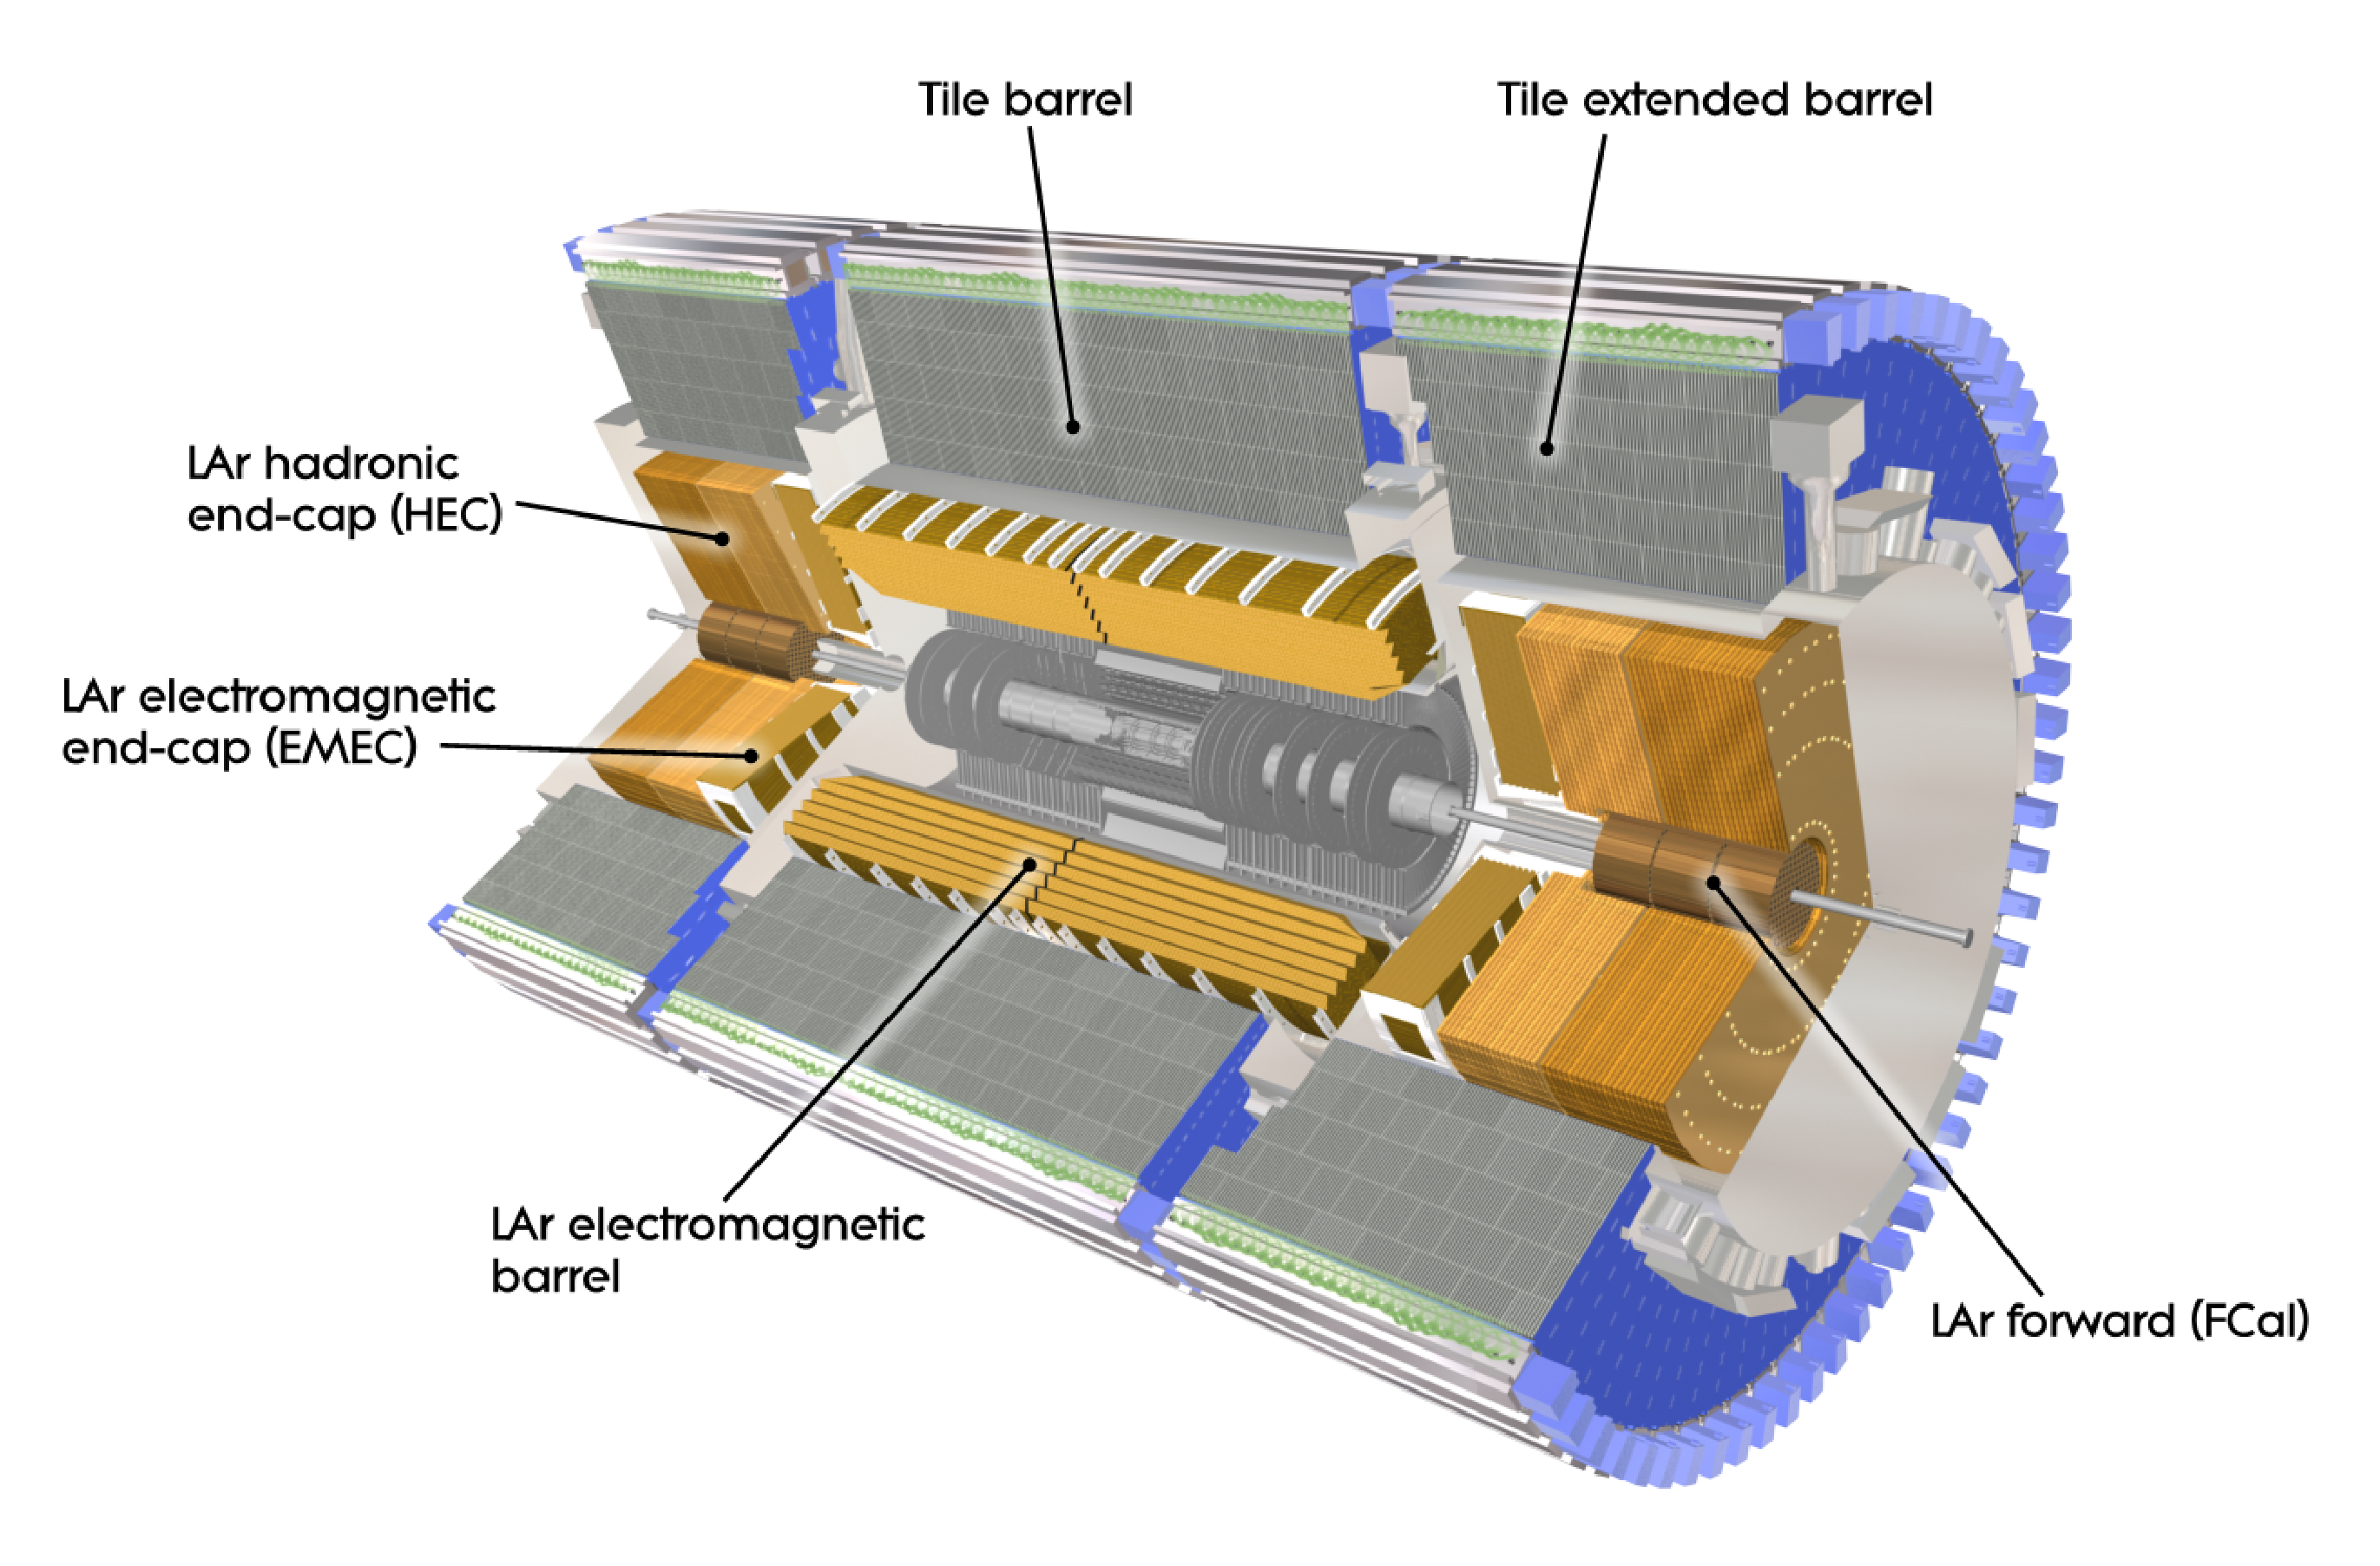
\includegraphics[width=0.995\textwidth]{ATLASdetector/Figures/Calorimeter.eps}
    }
  \end{center}
  \caption[Schematic view of the ATLAS calorimeter system.]{Schematic view of the ATLAS calorimeter system \protect\cite{Evans:2008zzb}.}
  \label{fig:CalorimetersSchema}
\end{figure}

The ATLAS calorimeters provide good containment for electromagnetic and hadronic showers. 
The thickness in the barrel of the EM calorimeter is greater than 22 radiation lengths ($X_0$), while it is greater than $24X_0$ in the end-caps.
An interaction length ($\lambda$) of active material of about 9.7 is found in the hadronic calorimeter barrel, while it increases up to about $10$ in the end-caps.
This thickness ensures an accurate $\met$ measurement.
Figure~\ref{fig:InteractionLengthCalo} shows the thickness in terms of interaction lengths of each layer of the ATLAS calorimeters versus $|\eta|$.

\begin{figure}[!ht]
  \begin{center}
    \mbox{
      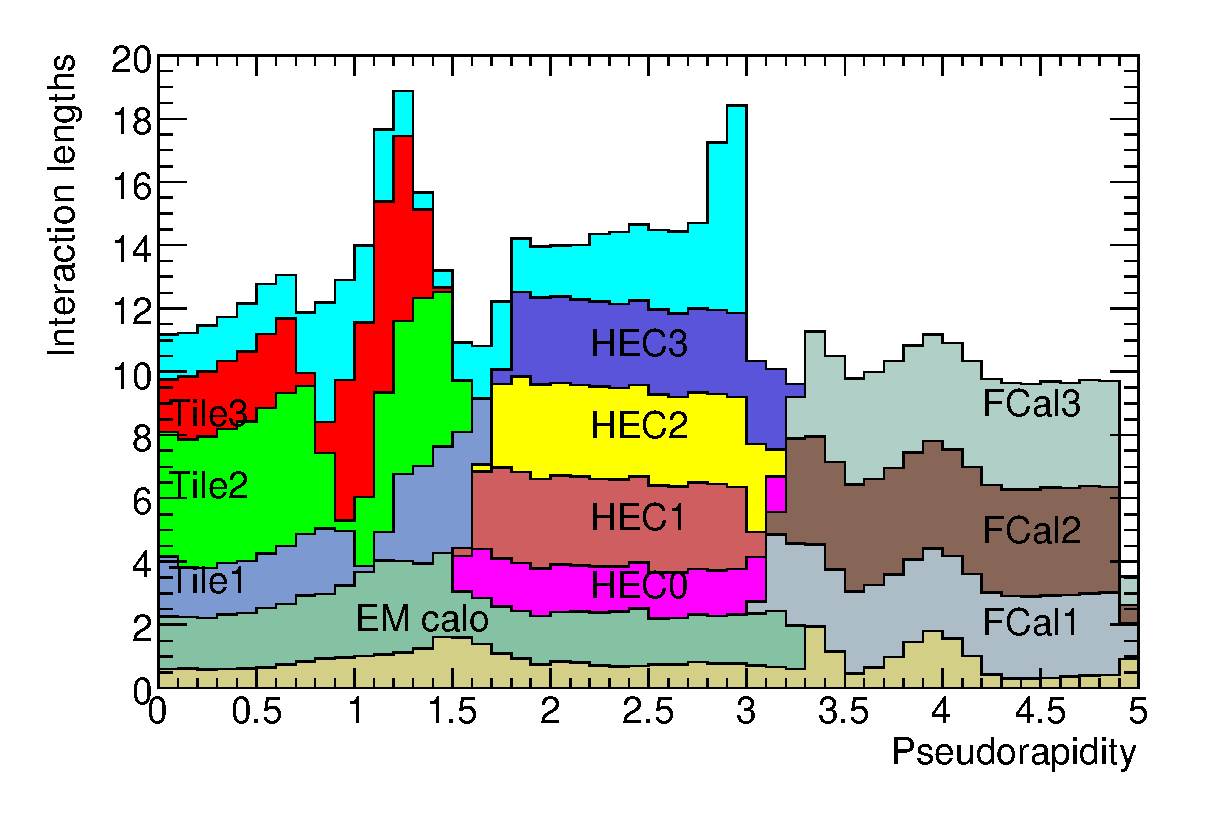
\includegraphics[width=0.995\textwidth]{ATLASdetector/Figures/CalorimeterRadiationLength.eps}
    }
  \end{center}
  \caption[Cumulative amount of material in the calorimeters and the first layer of the muon spectrometer.]{Cumulative amount of material, in units of interaction length, as a function of $|\eta|$, in front of the electromagnetic calorimeters, in the electromagnetic calorimeters themselves, in each hadronic compartment and the total amount at the end of the active calorimetry. Also shown for completeness is the total amount of material in front of the first active layer of the muon spectrometer (up to $|\eta|<3.0$) \protect\cite{Aad:2008zzm}.}
  \label{fig:InteractionLengthCalo}
\end{figure}


\subsubsection{Electromagnetic calorimeter}
    \label{subsubsec:LAr}

The electromagnetic calorimeter is a lead-LAr detector with accordion-shaped kapton electrodes and lead absorber plates over its full coverage.
Charged particles traversing the active material create couples of ions and electrons, that drift in opposite directions due to the presence of an electric field, and are collected by the Kapton electrodes. 
Different geometries for the Kapton electrodes have been used in order to minimize the calorimeter loss. 
For this reason, an accordion geometry has been used, which provides $\phi$ symmetry without azimutal cracks. 
Figure~\ref{fig:CalorimeterModules} (left) provides a schema of a LAr module.
The EM calorimeter is divided into a barrel part (EMB, $|\eta|<1.475$) and two end-caps (EMEC, $1.375<|\eta|<3.2$). 
All the LAr detectors are segmented transversely and divided in four layers in depth (a presampler and three layers), corresponding to a total of 182,468 cells.
The granularity of the different layers versus their $|\eta|$ coverage is shown in Table \ref{tab:LArGranularity}.
Located behind the EMEC is a copper-liquid argon hadronic end-cap calorimeter ($1.5<|\eta|<3.2$) and a copper/tungsten-liquid argon forward calorimeter, which will be explained in more detail in subsection~\ref{subsubsec:TileCal}.

\begin{table}[!ht]
  \begin{center}
    \begin{small}
      \setlength{\tabcolsep}{0.0pc}
      \begin{tabular*}{\textwidth}{@{\extracolsep{\fill}}ccccc}
        \noalign{\smallskip}\hline\hline\noalign{\smallskip}
                                     & \multicolumn{4}{c}{\textbf{EM calorimeter}} \\
                                     & \multicolumn{2}{c}{\textbf{Barrel}} & \multicolumn{2}{c}{\textbf{End-cap}} \\
                                     & $\Delta\eta \times \Delta\phi$ & $|\eta|$ & $\Delta\eta \times \Delta\phi$ & $|\eta|$ \\
        \noalign{\smallskip}\hline\noalign{\smallskip}
        Presampler                   & $0.025\times0.1$               & $<1.52$  &  $0.025\times0.1$              & 1.5-1.8 \\
        \noalign{\smallskip}\hline\noalign{\smallskip}
        \multirow{7}{*}{First layer} & $0.025/8\times0.1$             & $<1.40$  &  $0.050\times0.1$              & 1.375-1.425 \\
                                     & $0.025\times0.025$             & $1.40-1.475$  &  $0.025\times0.1$              & 1.425-1.5 \\
                                     &                                &          &  $0.025/8\times0.1$              & 1.5-1.8 \\
                                     &                                &          &  $0.025/6\times0.1$              & 1.8-2.0 \\
                                     &                                &          &  $0.025/4\times0.1$              & 2.0-2.4 \\
                                     &                                &          &  $0.025\times0.1$              & 2.4-2.5 \\
                                     &                                &          &  $0.1\times0.1$              & 2.5-3.2 \\
        \noalign{\smallskip}\hline\noalign{\smallskip}
        \multirow{3}{*}{Second layer}& $0.025\times0.025$             & $<1.40$  &  $0.050\times0.025$            & 1.375-1.425 \\
                                     & $0.075\times0.025$             & $1.40-1.475$  &  $0.025\times0.025$      & 1.425-2.5 \\
                                     &                                &          &  $0.1\times0.1$              & 2.5-3.2 \\
        \noalign{\smallskip}\hline\noalign{\smallskip}
        Third layer   & $0.050\times0.025$             & $<1.35$  &  $0.050\times0.025$              & 1.5-2.5 \\
        \noalign{\smallskip}\hline\hline\noalign{\smallskip}
      \end{tabular*}
    \end{small}
  \end{center}
  \caption{Granularity versus $\eta$ coverage of the different layers of the electromagnetic LAr calorimeter.}
  \label{tab:LArGranularity}
\end{table}

\begin{figure}[!ht]
  \begin{center}
    \mbox{
      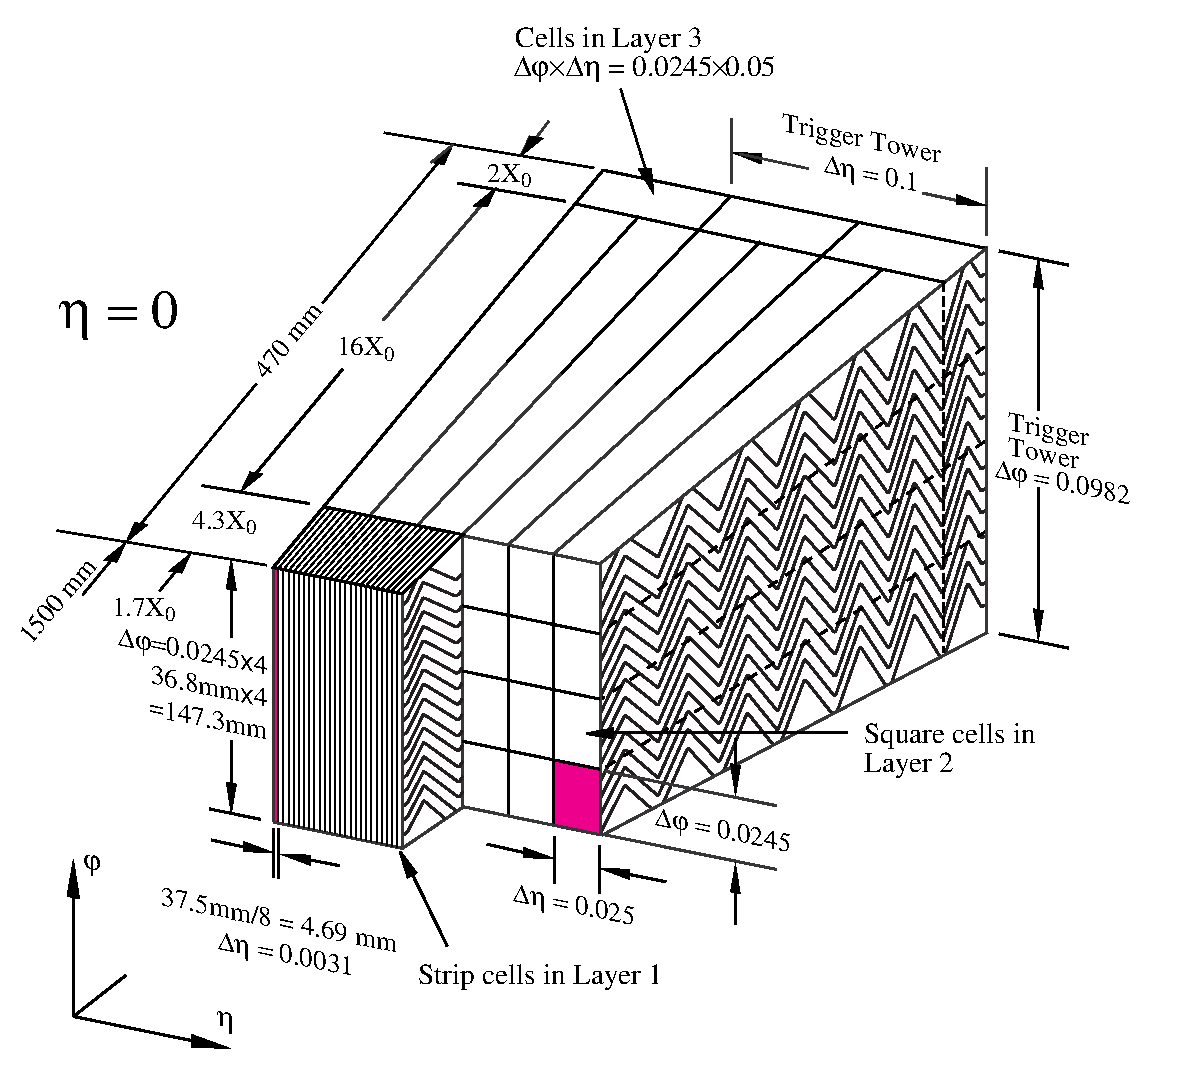
\includegraphics[width=0.495\textwidth]{ATLASdetector/Figures/LAr_Module.eps}
      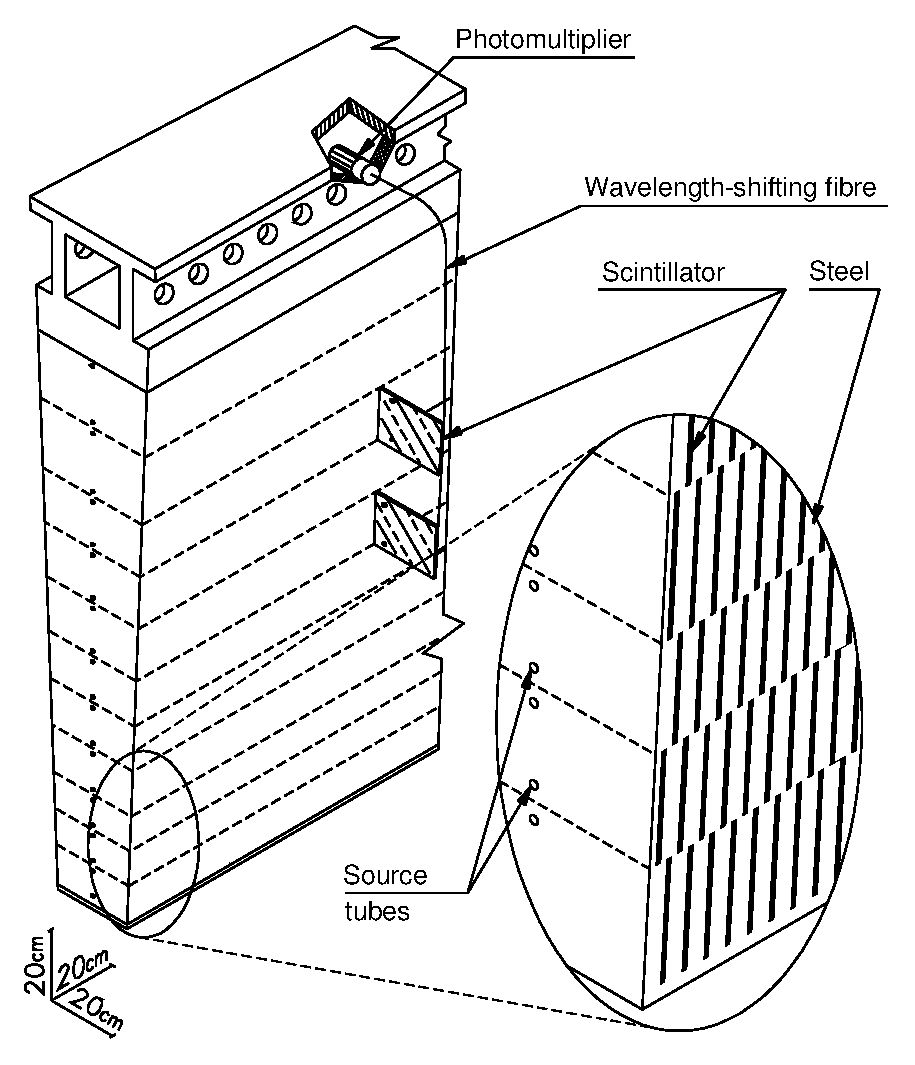
\includegraphics[width=0.495\textwidth]{ATLASdetector/Figures/TileCal_Module.eps}
    }
  \end{center}
  \caption[Schema of LAr and TileCal modules.]{Schema of LAr and TileCal modules~\cite{Aad:2010ai,Aad:2010af}.}
  \label{fig:CalorimeterModules}
\end{figure}

This calorimeter plays a central role in understanding the experimental signatures involving electrons, photons, $\met$, jets and taus.


\subsubsection{Hadronic calorimeter}
    \label{subsubsec:TileCal}

The hadronic calorimeter provides accurate energy and position measurements of isolated hadrons, taus and jets.
It also contributes in particle identification and in muon momentum reconstruction.
The central part of the calorimeter uses scintillating tiles technology, while the end-cap and forward hadronic calorimeter use the same LAr technology as the electromagnetic calorimeter discussed in the previous section.

The {\bf Tile Calorimeter} (TileCal) is placed directly surrounding the electromagnetic calorimeter and is divided into a barrel (LB, $|\eta|<1.0$) and two extended barrels (EB, $0.8<|\eta|<1.7$).
It uses plastic scintillator as the active material and low-carbon steel as the absorber.
Both the LB and the EB are segmented into 64 modules in $\phi$, corresponding to a $\Delta\phi$ granularity of $\unit[0.1]{radians}$.
Radially, each module is further segmented into three layers, which are approximately 1.5, 4.1 and 1.8 $\lambda$ thick for the barrel and 1.5, 2.6 and 3.3 for the extended barrel (as shown in Figure~\ref{fig:InteractionLengthCalo}).
The $\Delta\eta$ segmentation of each module is $0.1$ in the first two radial layers and $0.2$ in the third one.
Wavelength shifting fibers coupled to the tiles on either $\phi$ edge of the cells collect the produced light and are read out by two photomultiplier tubes (PMTs), each linked to one readout channel. 
Figure~\ref{fig:CalorimeterModules} (right) shows a schema of a TileCal module.
Furthermore, located on the inner radius surface of the extended barrel modules, the gap scintillators cover the region of $1.0<\eta<1.2$ while the crack scintillators are located on the front of the LAr end-cap and cover the region $1.2<\eta<1.6$.
Finally, 16 Minimum Bias Trigger Scintillators (MBTS) are located on the front face of the LAr end-cap cryostat and span an $\eta$ range of $2.12<\eta<3.85$.
The number of channels, cells and trigger outputs of the barrels, gap and crack and MBTS of the Tile calorimeter is summarized in Table~\ref{tab:TileCalCells}.
The TileCal related work developed during this PhD Thesis is collected in Appendix~\ref{app:DetectorWork}.

\begin{table}[!ht]
  \begin{center}
    \begin{small}
      \setlength{\tabcolsep}{0.0pc}
      \begin{tabular*}{\textwidth}{@{\extracolsep{\fill}}cccc}
        \noalign{\smallskip}\hline\hline\noalign{\smallskip}
                                     & \textbf{Channels} & \textbf{Cells} & \textbf{Trigger outputs} \\
        \noalign{\smallskip}\hline\noalign{\smallskip}
        Long barrel                  & 5760 & 2880 & 1152 \\
        Extended barrel              & 3564 & 1790 & 768 \\
        Gap and crack                & 480 & 480 & 128 \\
        MBTS                         & 32 & 32 & 32 \\
        \noalign{\smallskip}\hline\noalign{\smallskip}
        Total                        & 9836 & 5182 & 2080 \\
        \noalign{\smallskip}\hline\hline\noalign{\smallskip}
      \end{tabular*}
    \end{small}
  \end{center}
  \caption[Number of channels, cells and trigger outputs of the Tile Calorimeter.]{Number of channels, cells and trigger outputs of the Tile Calorimeter. The gap and crack and MBTS channels are readout in the extended barrel drawers \protect\cite{Aad:2010af}.}
  \label{tab:TileCalCells}
\end{table}

The {\bf Hadronic End-cap Calorimeter} (HEC) is a copper/liquid-argon hadronic end-cap calorimeter which consists of two independent wheels per end-cap, located directly behind the end-cap electromagnetic calorimeter.
They cover the region $1.5<|\eta|<3.2$, and each wheel is divided into two segments in depth.
The wheels are build from parallel copper plates as absorber, interleaved with LAr gaps providing the active medium.

The {\bf Forward Calorimeter} (FCal) is a copper/tungsten-liquid argon calorimeter. 
It is integrated into the end-cap cryostats, and it covers the region $3.1<|\eta|<4.9$.
The FCal consists of three modules per end-cap: the first is made of copper absorber, and is optimized for electromagnetic measurements, while the other two are made of tungsten and measure mainly the energy from hadronic interactions. 
All modules use LAr as active medium.

Table \ref{tab:TileGranularity} illustrates the granularity of each of the hadronic calorimeter layers versus the $|\eta|$ range.

\begin{table}[!ht]
  \begin{center}
    \begin{small}
      \setlength{\tabcolsep}{0.0pc}
      \begin{tabular*}{\textwidth}{@{\extracolsep{\fill}}ccccc}
        \noalign{\smallskip}\hline\hline\noalign{\smallskip}
                                     & \multicolumn{4}{c}{\textbf{Hadronic calorimeter}} \\
                                     & \multicolumn{2}{c}{\textbf{Scintillator tile}} & \multicolumn{2}{c}{\textbf{LAr hadronic}} \\
                                     & Barrel & Extended barrel & \multicolumn{2}{c}{End-cap} \\
        \noalign{\smallskip}\hline\noalign{\smallskip}
        $|\eta|$ coverage                            & $<1.0$         & 0.8-1.7        & 1.5-2.5        & 2.5-3.2 \\
         Number of layers                            & 3              & 3              & \multicolumn{2}{c}{4}       \\
        Granularity ($\Delta\eta \times \Delta\phi$) & $0.1\times0.1$ & $0.1\times0.1$ & \multirow{2}{*}{$0.1\times0.1$} & \multirow{2}{*}{$0.2\times0.2$} \\
        (last layer)                                 & $0.2\times0.1$ & $0.2\times0.1$ &                & \\ 
        \noalign{\smallskip}\hline\hline\noalign{\smallskip}
      \end{tabular*}
    \end{small}
  \end{center}
  \caption{Granularity versus $\eta$ coverage of the different layers of the hadronic calorimeter.}
  \label{tab:TileGranularity}
\end{table}


\subsection{Muon spectrometers}
    \label{subsec:MuonSpectrometers}

The Muon Spectrometer (MS) is surrounding the calorimeters, and is the most outer part of the ATLAS detector, as it is shown in Figure~\ref{fig:MuonSpectrometerSchema}. 
The MS has been designed to identify and measure high momentum muons and consists of four systems that make use of different technologies: Monitored Drift Tubes (MDT), Cathode Strip Chambers (CSC), Resistive Plate Chambers (RPC) and Thin Gap Chambers (TGC).
Table \ref{tab:MuonSpectrometerDetails} summarizes the properties of the muon spectrometer subsystems and their $\eta$ coverage.
The spectrometer is based on the magnetic deflection of muon tracks when they cross the magnetic field produced by the superconducting air-core toroid magnets.

\begin{table}[!ht]
  \begin{center}
    \begin{small}
      \setlength{\tabcolsep}{0.0pc}
      \begin{tabular*}{\textwidth}{@{\extracolsep{\fill}}ccccc}
        \noalign{\smallskip}\hline\hline\noalign{\smallskip}
                                     & \multicolumn{4}{c}{\textbf{Muon spectrometer}} \\
                                     & \textbf{MDT} & \textbf{CSC} & \textbf{RPC} & \textbf{TGC} \\
        \noalign{\smallskip}\hline\noalign{\smallskip}
        \multirow{2}{*}{$|\eta|$ coverage}     & $<2.7$          & \multirow{2}{*}{2.0-2.7} & \multirow{2}{*}{$<1.05$} & 1.05-2.7 \\
                                               & (innermost layer $<2.0$)          &  &  & (1.05-2.4 trigger) \\
         Number of chambers                            & 1150           & 32            & 606            & 3588       \\
         Number of channels                            & 354000         &310000         & 373000         & 318000     \\
         \multirow{2}{*}{Function}                     & Precision      & Precision& Triggering, & Triggering, \\
                                                       & tracking       & tracking & $\phi$-coordinate & $\phi$-coordinate \\
        \noalign{\smallskip}\hline\hline\noalign{\smallskip}
      \end{tabular*}
    \end{small}
  \end{center}
  \caption{Properties and $\eta$ coverage of the different Muon spectrometer subsystems.}
  \label{tab:MuonSpectrometerDetails}
\end{table}

\begin{figure}[!ht]
  \begin{center}
    \mbox{
      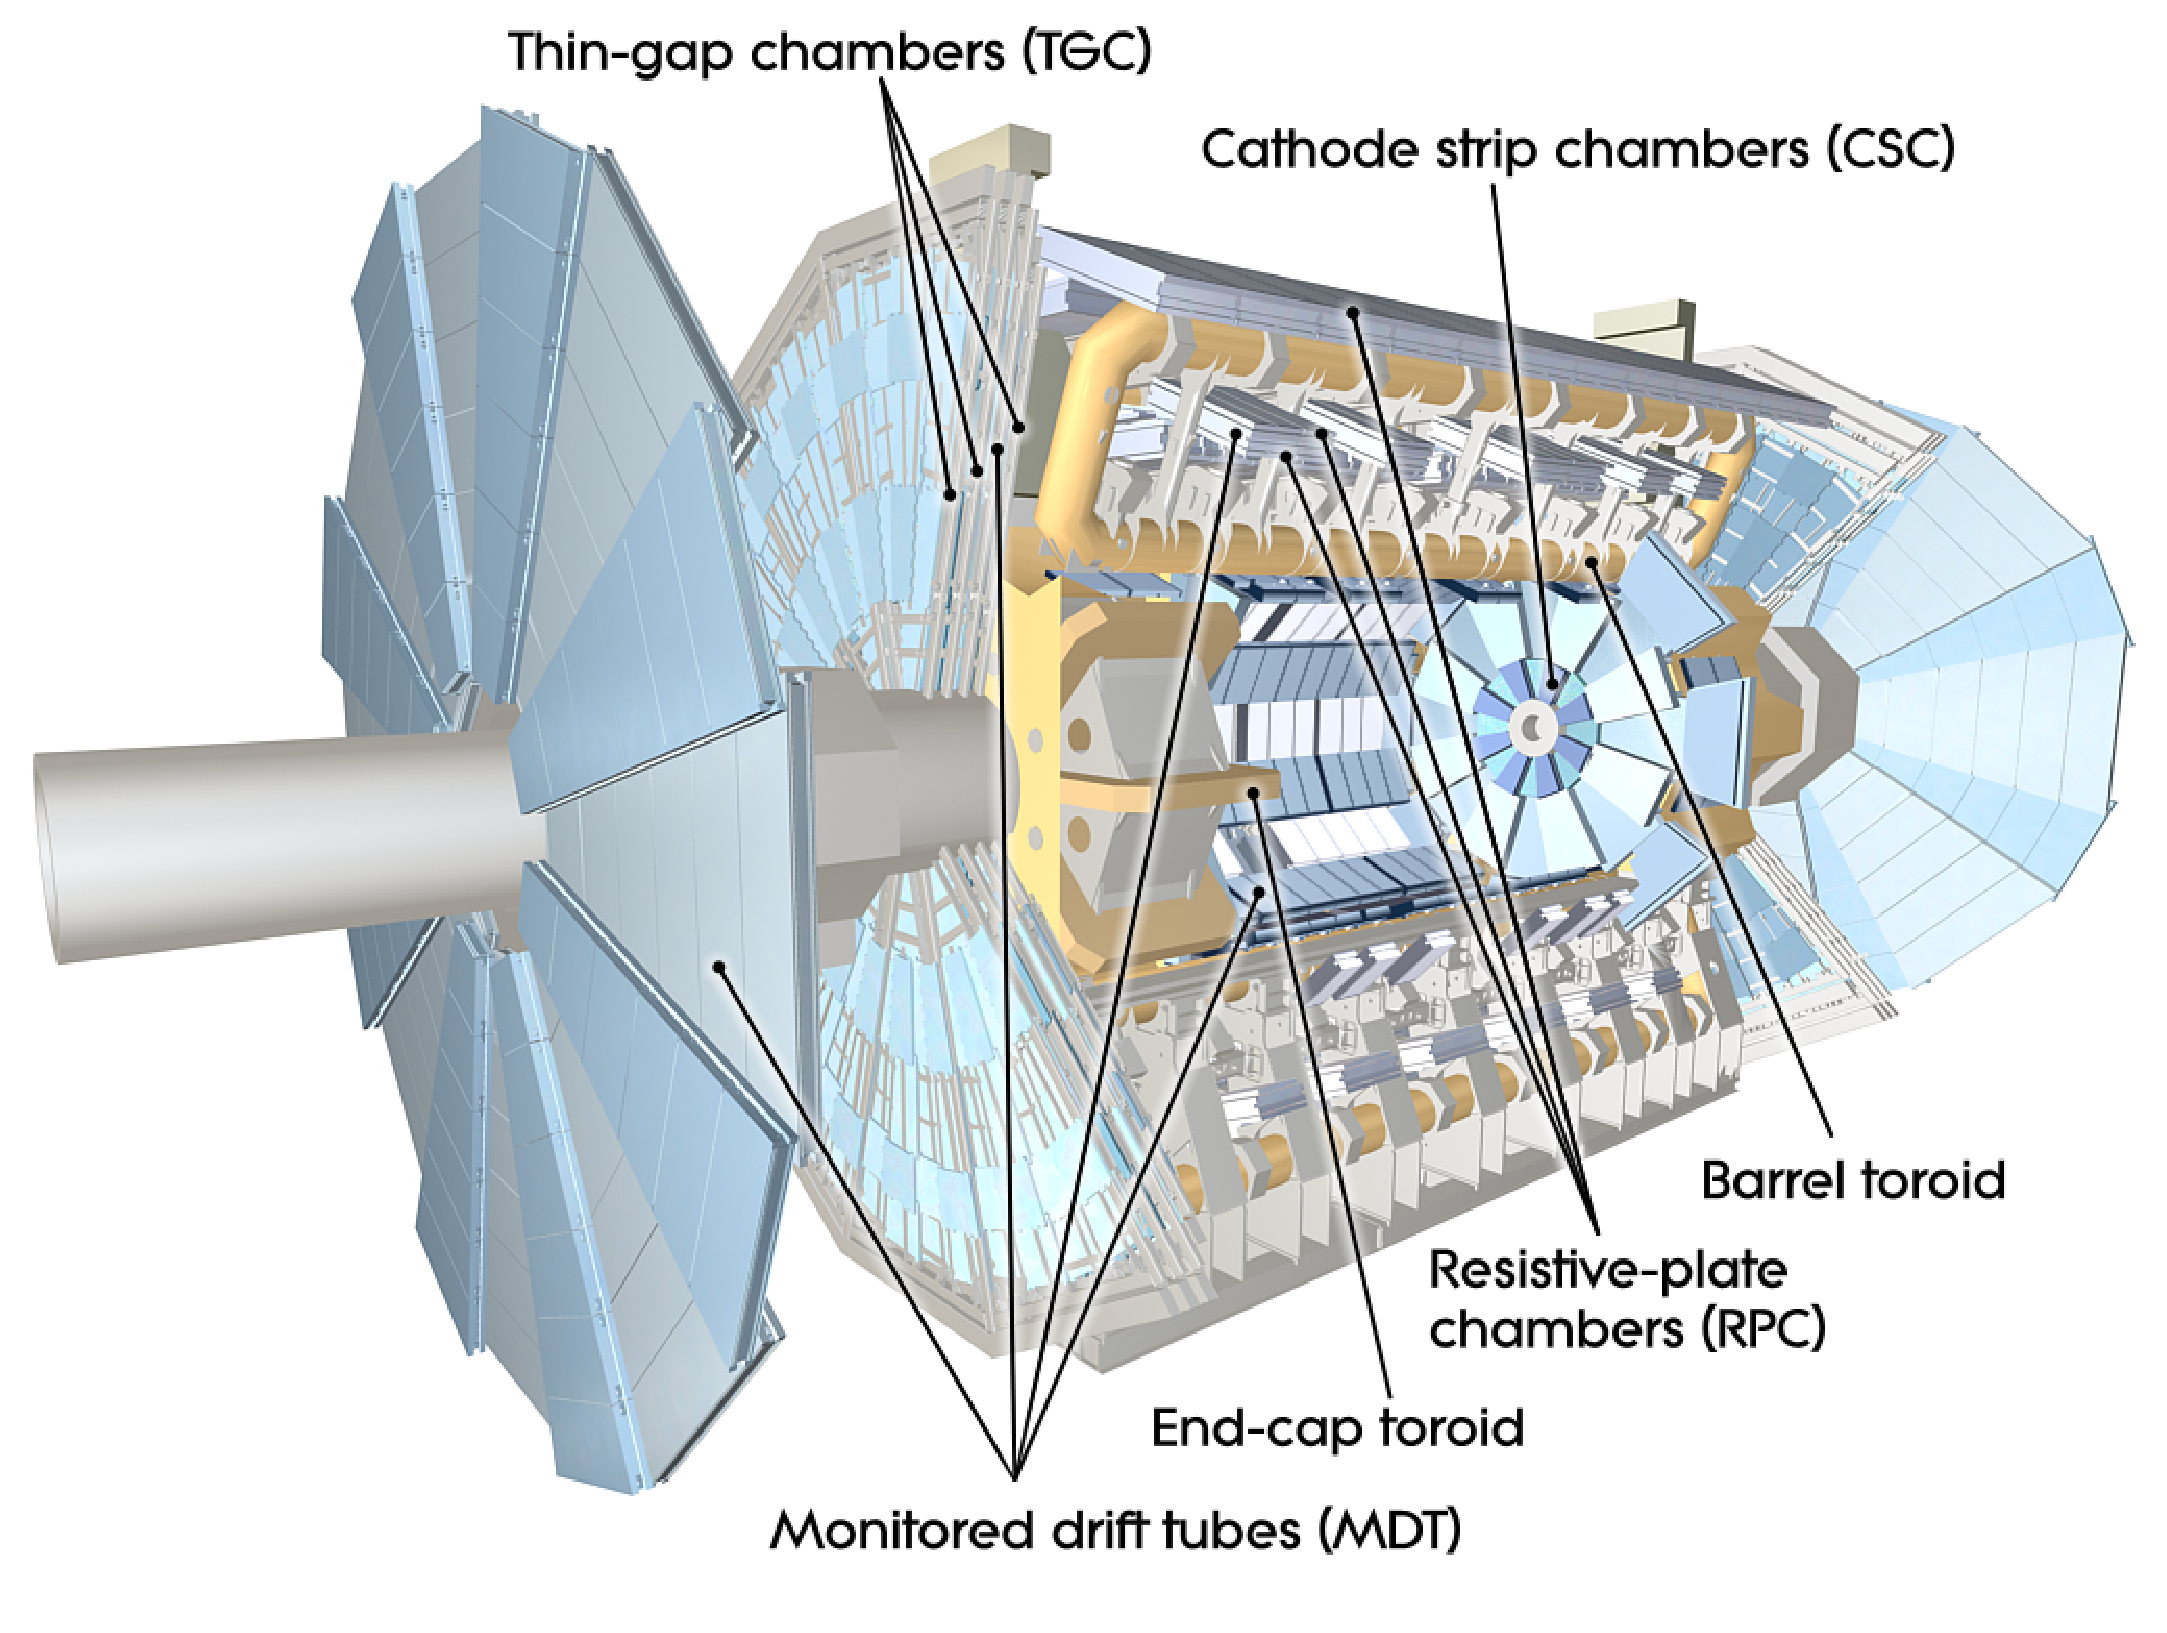
\includegraphics[width=0.995\textwidth]{ATLASdetector/Figures/MuonSystem.eps}
    }
  \end{center}
  \caption[Schematic view of the ATLAS muon spectrometer.]{Schematic view of the ATLAS muon spectrometer \cite{Evans:2008zzb}.}
  \label{fig:MuonSpectrometerSchema}
\end{figure}

The air-core toroid magnet is separated in three parts: one covering the central pseudo-rapidity range ($|\eta|<1.5$) producing a $\unit[0.5]{T}$ field, and the other two at higher pseudo-rapidity ($|\eta|>1.5$), generating a $\unit[1]{T}$ field.
Each of the magnets consist of eight coils assembled radially around the beam axis, to create a magnetic field almost orthogonal to the muon trajectories and bends them along the $\theta$ angle.

The {\bf Monitor Drifted Tubes} provide a precision coordinate measurement in the bending direction of the air-core toroidal magnet, and therefore provide the  muon momentum measurement for $|\eta|<2.7$.
The basic detection element is a cylindrical aluminum drift tube filled with gas and a central wire at a high potential. The muons passing through the tubes ionize the gas and produce charges that are collected on the wire.

The {\bf Cathode Strip Chambers} are used at high pseudo-rapidities to help confronting the demanding rate and background conditions.
They are multiwire proportional chambers with cathodes segmented into strips.

The {\bf Resistive Plate Chambers} (in the barrel) and the {\bf Thin Gap Chambers} (in the end-caps) are trigger chambers that can provide bunch-crossing identification, well-defined $\pt$ thresholds and they can measure the muon coordinate in the $\phi$ direction.


\subsection{Trigger system}
    \label{subsec:TriggerSystem}

The purpose of the trigger system is to reduce the input rate from several MHz to about $\unit[400]{Hz}$ for recording and offline processing.
This limit is equivalent to an average data rate of about $\unit[300]{MB/s}$, which is the maximum that the computer resources and the offline storage can handle.
For each bunch crossing, the trigger system verifies if at least one of hundreds of conditions (triggers) are satisfied.
Most of them are based on identifying combinations of candidate physics objects such as electrons, muons or jets, but there are also triggers for inelastic $\pp$ collisions (minimum bias) and triggers based on global event properties, such as $\sum\et$ or $\met$.

The system has three levels; the first level (L1) is a hardware-based system using information from the calorimeter and muon sub-detectors. 
The second (L2) and the third (Event Filter, EF) together are software-based systems that use information from all sub-detectors. 
They are called the High Level Trigger (HLT).

\begin{figure}[!ht]
  \begin{center}
    \mbox{
      \includegraphics[width=0.995\textwidth]{ATLASdetector/Figures/TriggerSystem.eps}
    }
  \end{center}
  \caption[Schema of the ATLAS trigger system.]{Schema of the ATLAS trigger system~\protect\cite{Aad:2012xs}.}
  \label{fig:TriggerSchema}
\end{figure}

Figure~\ref{fig:TriggerSchema} shows a schema of the ATLAS trigger system.
Detector signals are stored in front-end pipelines pending a decision from the L1 trigger system, which is implemented in fast electronics in order to minimize the latency time.
In addition to performing the first selection step, the L1 triggers identify Regions of Interest (RoIs) within the detector to be investigated by the HLT.
It is designed to reduce the rate to a maximum of $\unit[75]{kHz}$.
The HLT consists of farms of processors connected by fast dedicated networks.
When an event is accepted by the L1 trigger, data from each detector are transferred to the detector-specific Readout Buffers (ROB), which store the event in fragments pending the L2 decision.
The L2 selection is based on fast custom algorithms processing partial event data within the RoIs identified by L1.
The L2 processors request data corresponding to detector elements inside each RoI, reducing the amount of data to be transferred.
The L2 triggers reduce the rate to approximately $\unit[3]{kHz}$ with an average processing of $\unit[40]{ms}$ per event.
Finally the EF is based on offline algorithms and it is designed to reduce the rate up to $\unit[400]{Hz}$. 
It uses the full information of the events passing the L2.


\subsection{Luminosity measurement}
    \label{subsec:LuminosityMeasurement}

An accurate measurement of the luminosity is a key component for all physics analyses. 
For cross section measurements, the uncertainty on the delivered luminosity is one of the major systematic uncertainties, but also searches for new physical phenomena beyond the Standard Model rely on accurate information about the delivered luminosity to evaluate background levels and determine sensitivity to the signatures of new phenomena.
The ATLAS luminosity is determined with a number of sub-detectors, using different methods and algorithms \cite{Aad:2013ucp}.

The instantaneous luminosity, $\InstLumi$, can be expressed in terms of accelerator parameters, as:

\begin{equation}
  \InstLumi = \frac{n_{b} f_{r} n_{1} n_{2}}{2\pi \Sigma_{x} \Sigma_{y}}, 
  \label{LumiDefinitionAccelerator}
\end{equation}

\noindent where $n_{1}$ and $n_{2}$ are the bunch populations (protons per bunch) in beams~1 and~2 respectively, $f_{r}$ is the revolution frequency of the LHC, $n_{b}$ are the bunch pairs colliding in each revolution and $\Sigma_{x}$ and $\Sigma_{y}$ characterize the horizontal and vertical convolved beam widths, extracted in a {\emph van der Meer} (vdM) scan\footnote{Also known as beam-separation scan}.
In a vdM scan, the observed event rate is recorded while scanning the two beams across each other first in the horizontal ($x$) and then in the vertical ($y$) directions. This yields two bell-shaped curves, with the maximum rate at zero separation, from which the $\Sigma_{x}$ and $\Sigma_{y}$ values can be extracted.
Then, the total absolute luminosity can be computed with Equation~\ref{LumiDefinitionAccelerator}.

The luminosity can be re-written as:

\begin{equation}
  \InstLumi = \frac{R_{\text{inel}}}{\sigma_{\text{inel}}} = 
  \frac{\averageIntXing n_b f_r}{\sigma_{\text{inel}}} = 
  \frac{\averageIntXing_{\text{vis}} n_b f_r}{\sigma_{\text{vis}}}, 
  \label{LumiDefinition}
\end{equation}

\noindent where $R_{\text{inel}}$ is the rate of inelastic collisions, $\sigma_{\text{inel}}$ is the $\pp$ inelastic cross-section, $\averageIntXing$ is the average number of interactions per bunch crossing (BC) and $\sigma_{\text{vis}} = \epsilon\sigma_{\text{inel}}$, where $\epsilon$ is the efficiency of a particular detector and algorithm.

By measuring simultaneously the peak collision rate (at zero beam separation), $\averageIntXing_{\text{vis}}^{\text{MAX}}$, and the corresponding peak absolute luminosity, $\InstLumi^{\text{MAX}}$ (using Eq. \ref{LumiDefinitionAccelerator}), the constant $\sigma_{\text{vis}} = \epsilon\sigma_{\text{inel}}$ can be determined by:

\begin{equation}
  \sigma_{\text{vis}} = \averageIntXing_{\text{vis}}^{\text{MAX}} \frac{n_{b} f_{r}}{\InstLumi^{\text{MAX}}}.
  \label{LumiVisibleXSection}
\end{equation}

Therefore, after the calibrations from the vdM scan, the ATLAS luminosity can be directly computed with Equation~\ref{LumiDefinition}, once $\averageIntXing_{\text{vis}}$ has been determined.
In order to measure this quantity with a sub-detector, ATLAS primarily uses event counting algorithms for which the number of events that satisfies a given criteria are compared to the total number of bunch crossings.
In a vdM scan $\averageIntXing_{\text{vis}} \muchless 1$, and the average number of visible inelastic interactions per BC is given by the expression:

\begin{equation}
  \averageIntXing_{\text{vis}} = \frac{N}{N_{\text{BC}}},
  \label{LumiVisibleMuSmall}
\end{equation}

\noindent where $N$ is the number of events that satisfies the event selection criteria during a given time interval and $N_{\text{BC}}$ is the total number of bunch crossings during the same interval.
